% ============================================================================
% Lecture 02 (B01): Why Deep Learning for Economics and Finance?
% Deep Learning for Solving and Estimating Dynamic Models in Economics and Finance
% Course author: Simon Scheidegger
% ============================================================================

\documentclass[aspectratio=169,11pt]{beamer}

% ---------- Theme and colors ----------
\usecolortheme{dove}
\setbeamertemplate{navigation symbols}{}
\setbeamertemplate{footline}{%
  \hfill\usebeamerfont{page number in head/foot}%
  \usebeamercolor[fg]{normal text}%
  \insertframenumber\,/\,\inserttotalframenumber\kern1em\vskip4pt}
\setbeamerfont{frametitle}{size=\huge}

% ---------- Packages ----------
\usepackage[utf8]{inputenc}
\usepackage[T1]{fontenc}
\usepackage{amsmath,amssymb,amsfonts}
\usepackage{bm}
\usepackage{graphicx}
\usepackage{tikz}
\usetikzlibrary{shapes,arrows.meta,positioning,calc,fit,backgrounds,patterns,decorations.pathreplacing}
\usepackage{pgfplots}
\pgfplotsset{compat=1.18}
\usepackage{booktabs}
\usepackage{hyperref}
\usepackage{multicol}
\usepackage{xcolor}
\usepackage{algorithm}
\usepackage{algorithmic}

% ---------- Custom colors ----------
\definecolor{uzhblue}{rgb}{0,0,0.5}
\definecolor{uzhgreylight}{RGB}{236,238,241}
\definecolor{uzhgreydark}{RGB}{81,86,94}
\definecolor{harvardcrimson}{RGB}{153,0,0}
\definecolor{unil@blue}{RGB}{0,140,204}
\definecolor{unil@black}{RGB}{35,31,32}
\definecolor{darkgreen}{RGB}{0,100,0}
\definecolor{darkred}{RGB}{139,0,0}
\definecolor{softblue}{RGB}{70,130,180}
\definecolor{softorange}{RGB}{230,159,0}
\definecolor{softgreen}{RGB}{0,158,115}

% ---------- Set beamer colors ----------
\setbeamercolor{frametitle}{bg=uzhgreylight, fg=uzhblue}
\setbeamercolor{title}{fg=uzhblue}
\setbeamercolor{structure}{fg=uzhblue}
\setbeamercolor{block title}{bg=unil@blue, fg=white}
\setbeamercolor{block body}{bg=uzhgreylight}
\setbeamercolor{block title alerted}{bg=darkred,fg=white}
\setbeamercolor{block body alerted}{bg=red!5}
\setbeamercolor{block title example}{bg=darkgreen,fg=white}
\setbeamercolor{block body example}{bg=green!5}
\setbeamercolor{item}{fg=unil@black}
\setbeamercolor{normal text}{fg=unil@black}

% ---------- Emphasis and hyperlinks ----------
\newcommand{\emphc}[1]{\textcolor{harvardcrimson}{#1}}
\hypersetup{colorlinks,linkcolor=harvardcrimson,urlcolor=harvardcrimson}

% ---------- Math commands ----------
\newcommand{\x}{\bm{x}}
\newcommand{\w}{\bm{w}}
\newcommand{\bb}{\bm{b}}
\newcommand{\z}{\bm{z}}
\newcommand{\W}{\bm{W}}
\newcommand{\X}{\bm{X}}
\renewcommand{\a}{\bm{a}}
\newcommand{\R}{\mathbb{R}}
\newcommand{\E}[1]{\mathbb{E}\!\left[#1\right]}
\DeclareMathOperator*{\argmin}{arg\,min}
\DeclareMathOperator*{\argmax}{arg\,max}

\title[Lecture 02 (B01)]{Lecture 02 (B01): Introduction to deep learning}
\subtitle{From basic ML through DNNs to sequence models for economic time series}
\author{Simon Scheidegger}
\institute{HEC, University of Lausanne}
\date{}
\begin{document}

{\setbeamercolor{background canvas}{bg=uzhgreylight}
\begin{frame}
\titlepage
\end{frame}
}

% --- About-this-lecture orientation ---

% ============================================================================
% PART 1: SETTING THE STAGE
% ============================================================================

% --- Slide 1: Title ---
{\setbeamercolor{background canvas}{bg=uzhgreylight}
\begin{frame}
\titlepage
\end{frame}
}

% --- Slide 2: Course Overview ---
\begin{frame}{Course Overview}
\footnotesize
\begin{columns}[T]
\column{0.48\textwidth}
\textbf{Discrete-time block (Lectures 02--17)}
\begin{itemize}
    \item Lectures 02--05~~Intro to ML \& Deep Learning
    \item Lectures 06--10~~Deep Equilibrium Nets (DEQNs)
    \item Lectures 11--12~~IRBC, NAS \& Loss Normalization
    \item Lectures 13--17~~OLG, Young's method, Krusell--Smith, sequence-space DEQNs
\end{itemize}

\column{0.48\textwidth}
\textbf{Toolkits and continuous-time block (Lectures 18--30)}
\begin{itemize}
    \item Toolkit T1 / T2~~Agentic Programming (AI for Research)
    \item Lectures 18--21~~PINNs \& CT Heterogeneous Agents (HJB+KFE)
    \item Lectures 22--26~~Surrogates, GPs, Deep Kernels, SMM
    \item Lectures 27--30~~Climate Economics, IAMs \& Deep UQ
\end{itemize}
\end{columns}
\normalsize

\vspace{0.6cm}
\begin{center}
\textbf{All materials:}~~\url{https://github.com/sischei/Deep_Learning_for_Solving_And_Estimating_Dynamic_Economic_Models}\\[4pt]
\end{center}
\end{frame}

% --- Slide 3: Roadmap ---
\begin{frame}{Roadmap of This Lecture}
\begin{columns}[T]
\column{0.48\textwidth}
\textbf{Machine Learning Foundations}
\begin{itemize}
    \item What is ML?  Supervised, unsupervised, RL
    \item The three-step ML recipe
\end{itemize}

\vspace{0.5em}
\textbf{From Perceptrons to Deep Nets}
\begin{itemize}
    \item The perceptron and activation functions
    \item Multi-layer networks and universal approximation
\end{itemize}

\column{0.48\textwidth}
\textbf{Training, Generalization \& Practice}
\begin{itemize}
    \item Losses, gradient descent, backpropagation
    \item Regularization, optimizers, software ecosystem
\end{itemize}

\vspace{0.5em}
\textbf{Sequence Models}
\begin{itemize}
    \item RNNs, LSTMs, attention, transformers
    \item What matters for economic time series
\end{itemize}
\end{columns}
\end{frame}

% --- Slide 4: The Rise of Neural Networks ---
\begin{frame}{The Rise of Neural Networks}
\begin{center}
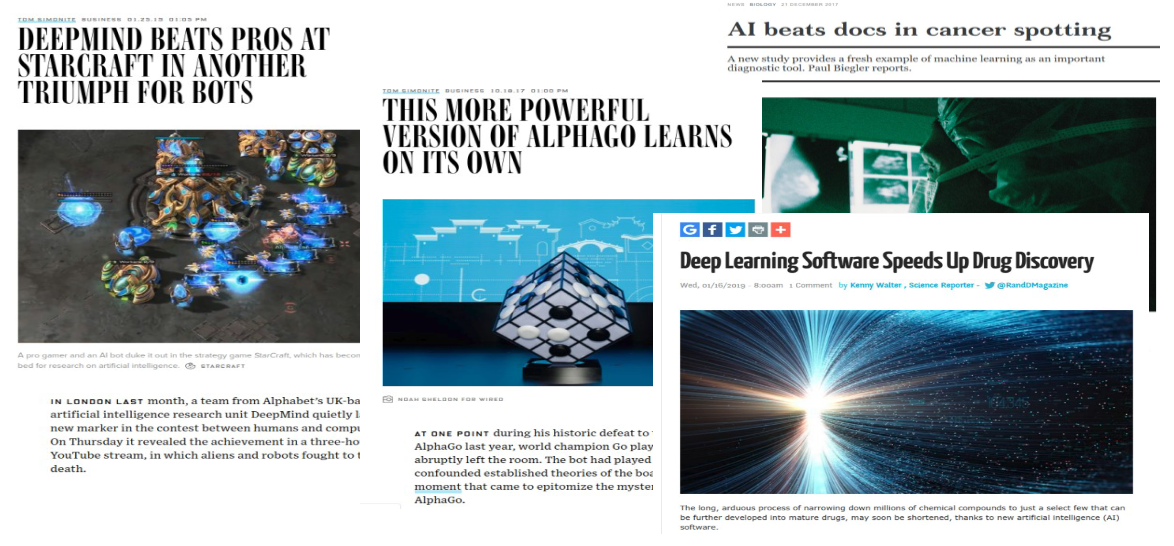
\includegraphics[width=\textwidth]{figures/rise.png}
\end{center}
\end{frame}

% --- Slide 5: AI Music Generation ---
\begin{frame}{AI Music Generation}
\begin{columns}[T]
\column{0.45\textwidth}
\begin{center}

\includegraphics[width=\textwidth]{figures/musenet.png}
\end{center}

\column{0.52\textwidth}
\textbf{OpenAI MuseNet} can generate 4-minute musical compositions with 10 different instruments, combining styles from country to Mozart to the Beatles.

\vspace{0.4cm}
Deep learning enables machines to:
\begin{itemize}
    \item Compose music in different genres
    \item Combine multiple instrumental tracks
    \item Learn long-range structure in sequences
\end{itemize}
\end{columns}
\end{frame}

% --- Slide 6: Style Transfer ---
\begin{frame}{Neural Style Transfer}
\begin{center}
\begin{columns}[c]
\column{0.32\textwidth}
\begin{center}
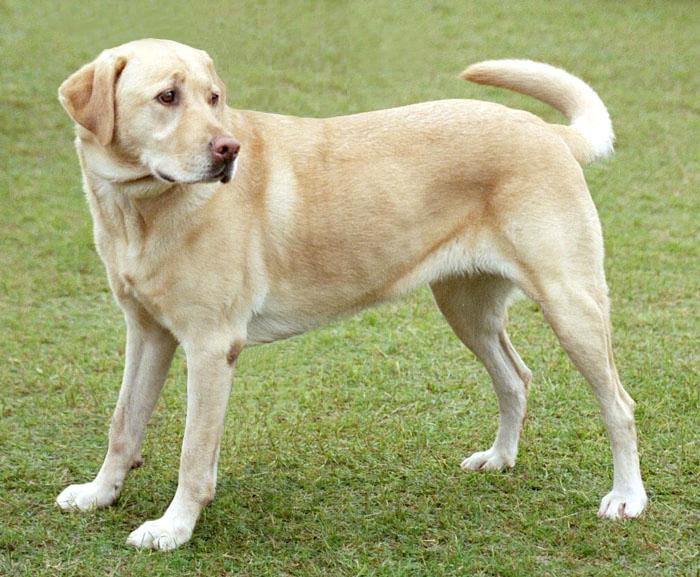
\includegraphics[width=\textwidth]{figures/dog1.png}\\[4pt]
{\small Content image}
\end{center}
\column{0.32\textwidth}
\begin{center}
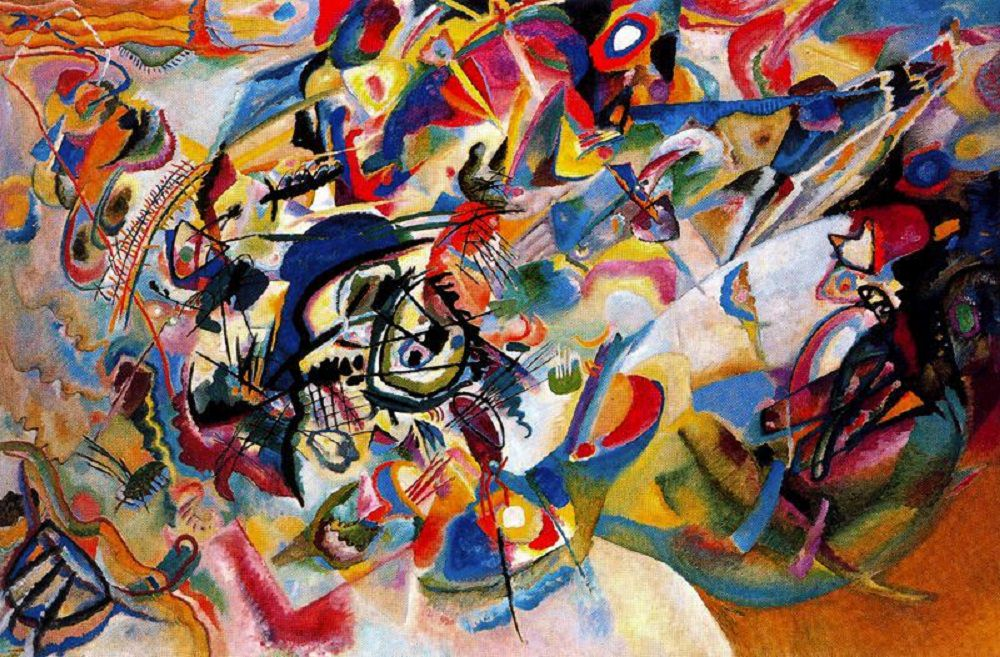
\includegraphics[width=\textwidth]{figures/kandinsky.png}\\[4pt]
{\small Style image (Kandinsky)}
\end{center}
\column{0.32\textwidth}
\begin{center}
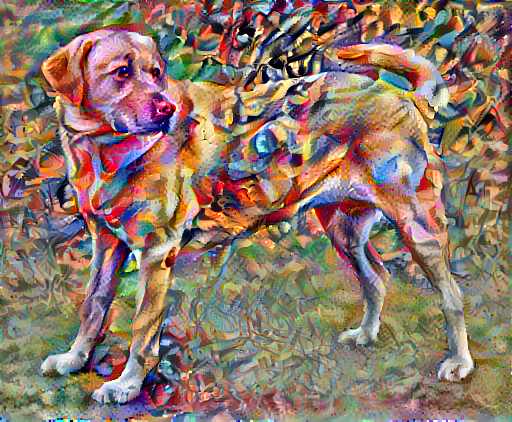
\includegraphics[width=\textwidth]{figures/dog2.png}\\[4pt]
{\small Result}
\end{center}
\end{columns}
\end{center}

\vspace{0.3cm}
{\small Gatys, Ecker \& Bethge (2015): a neural network separates and recombines content and style of images.}
\end{frame}

% --- Slide 7: Self-Driving Cars ---
\begin{frame}{Self-Driving Cars}
\begin{columns}[T]
\column{0.48\textwidth}
\begin{center}
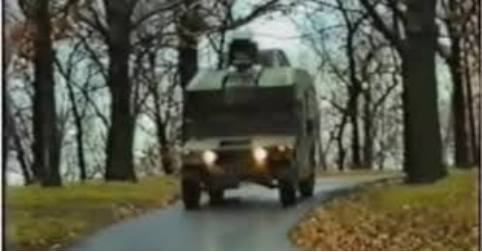
\includegraphics[width=\textwidth]{figures/alvinn.png}\\[4pt]
{\small \textbf{ALVINN} (1989), one of the first autonomous vehicles, using a simple neural network.}
\end{center}

\column{0.48\textwidth}
\begin{center}
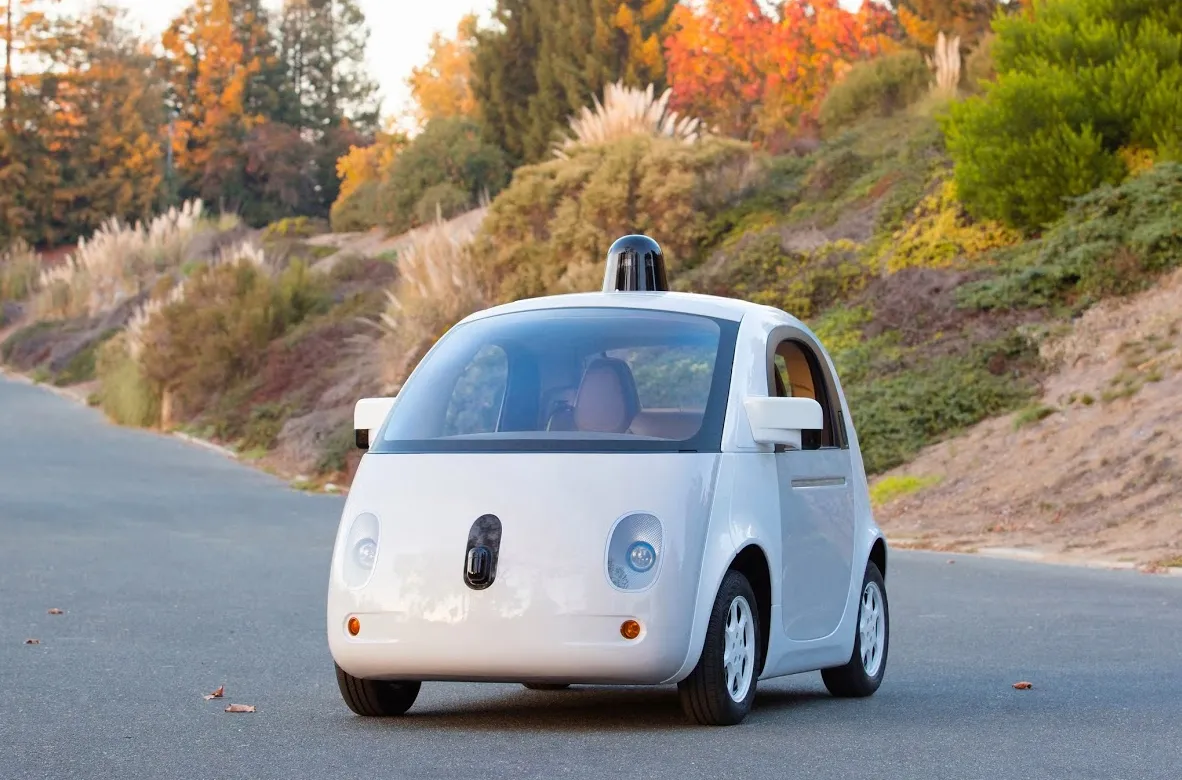
\includegraphics[width=\textwidth]{figures/waymo.png}\\[4pt]
{\small \textbf{Waymo} (2017+), deep learning for perception, prediction, and planning.}
\end{center}
\end{columns}
\end{frame}

% --- Slide 8: Two-Legged Robots ---
\begin{frame}{Two-Legged Robots}
\begin{columns}[T]
\column{0.48\textwidth}
\begin{center}
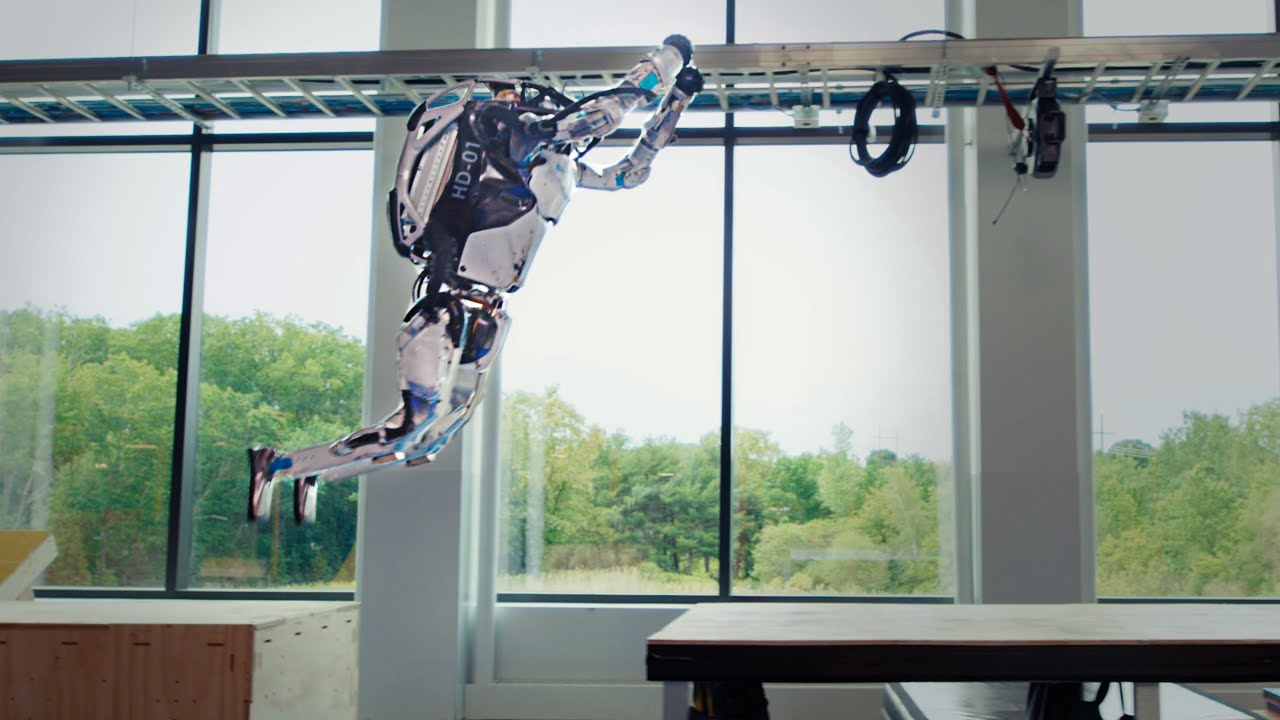
\includegraphics[width=0.9\textwidth]{figures/atlas.png}\\[4pt]
{\small \textbf{Boston Dynamics Atlas}\\
\url{https://www.bostondynamics.com/atlas}}
\end{center}

\column{0.48\textwidth}
\begin{center}
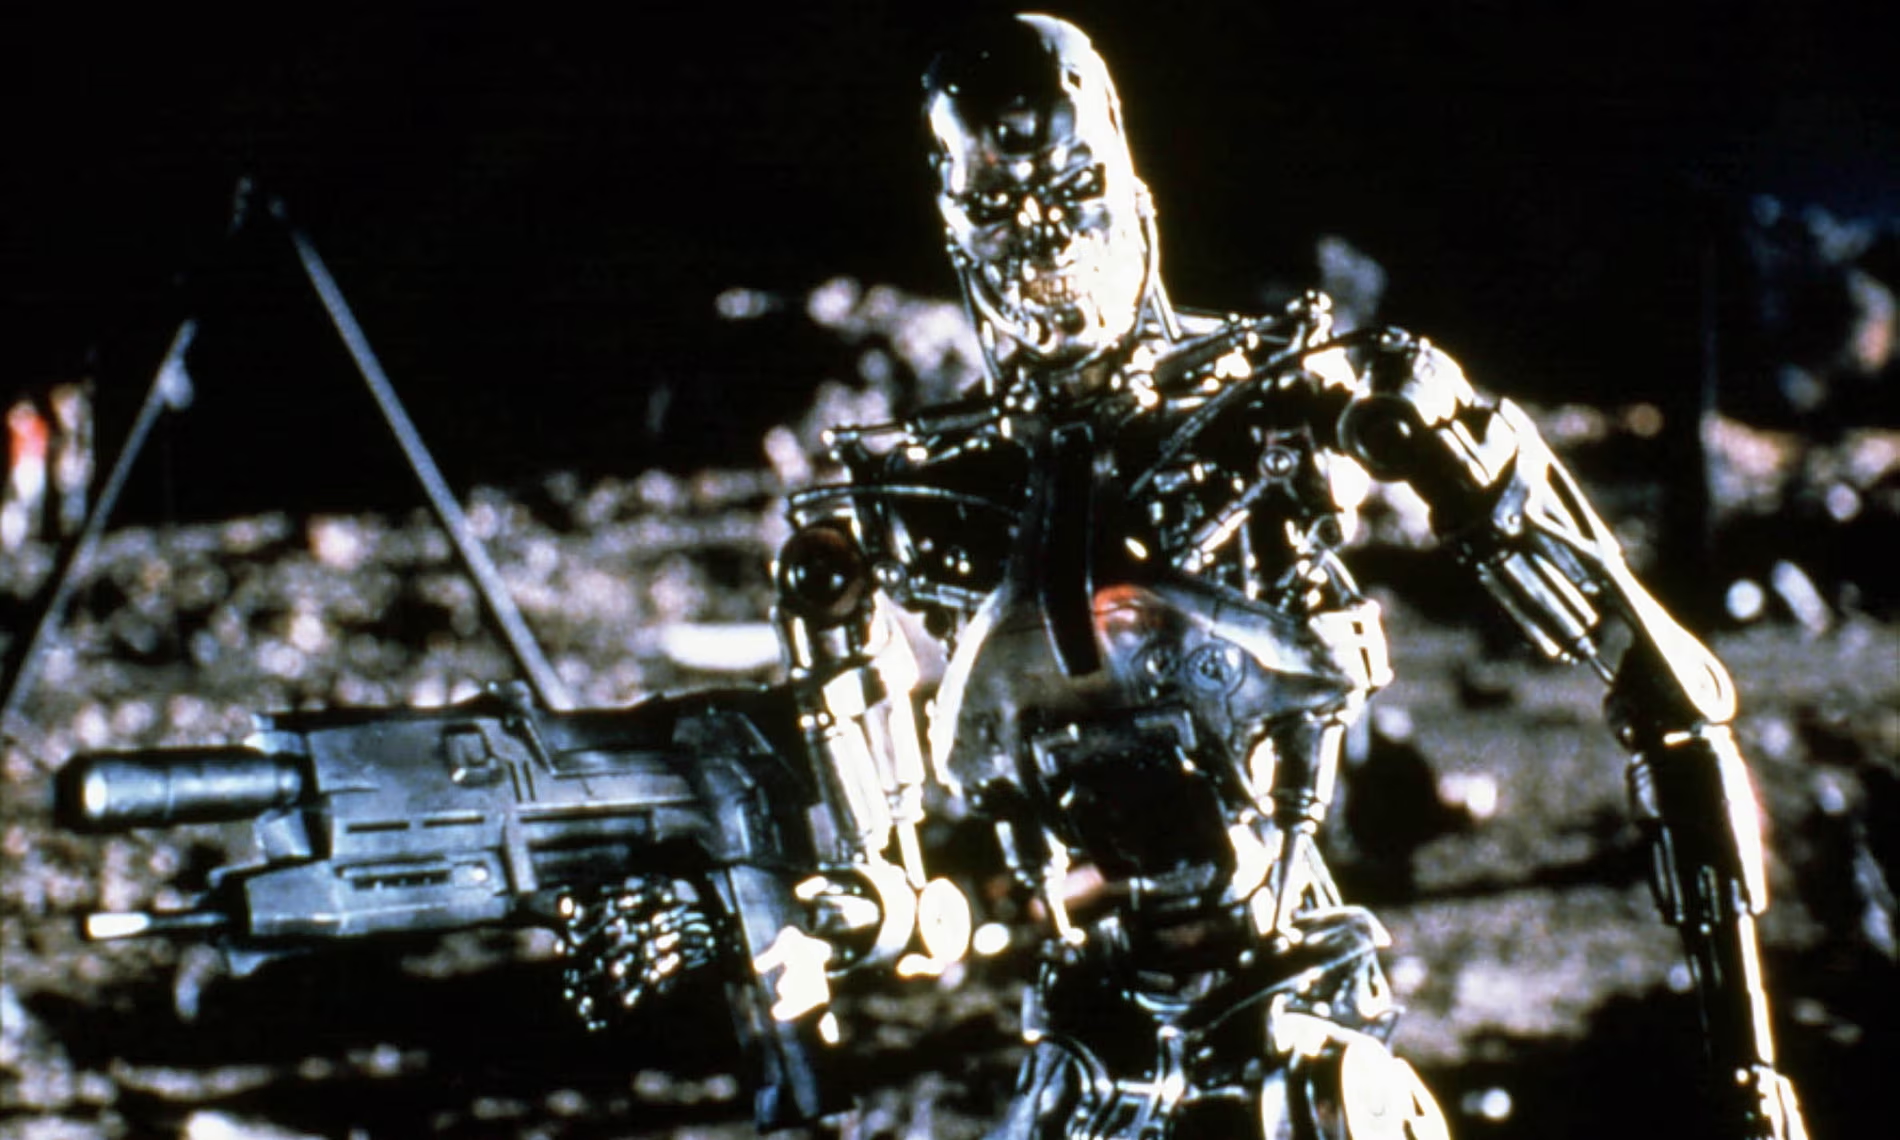
\includegraphics[width=0.9\textwidth]{figures/terminator.png}\\[4pt]
{\small Science fiction meets reality, deep reinforcement learning enables humanoid locomotion.}
\end{center}
\end{columns}
\end{frame}

% --- Slide 9: Coloring Old Movies ---
\begin{frame}{Coloring Old Movies}
\begin{columns}[T]
\column{0.48\textwidth}
\begin{center}
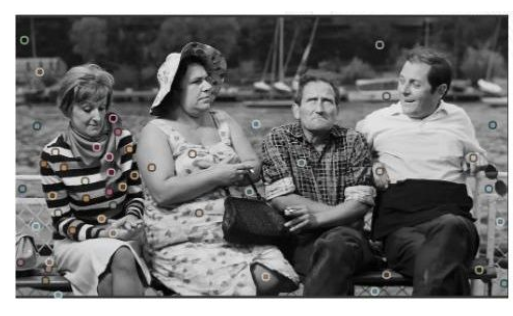
\includegraphics[width=\textwidth]{figures/bw.png}\\[4pt]
{\small Original black-and-white frame}
\end{center}

\column{0.48\textwidth}
\begin{center}
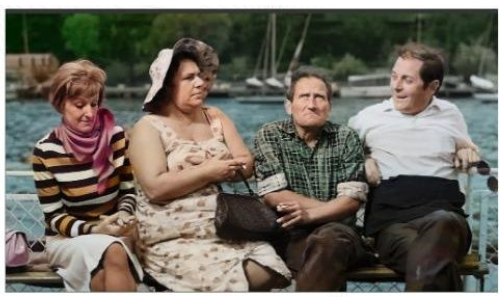
\includegraphics[width=\textwidth]{figures/color.png}\\[4pt]
{\small Automatic colorization using deep learning}
\end{center}
\end{columns}

\vspace{0.3cm}
{\small Deep neural networks learn to predict plausible colors from grayscale input, trained on millions of color images.}
\end{frame}

% --- Slide 10: A Timeline of Deep Learning ---
\begin{frame}{A Timeline of Deep Learning}
\begin{center}
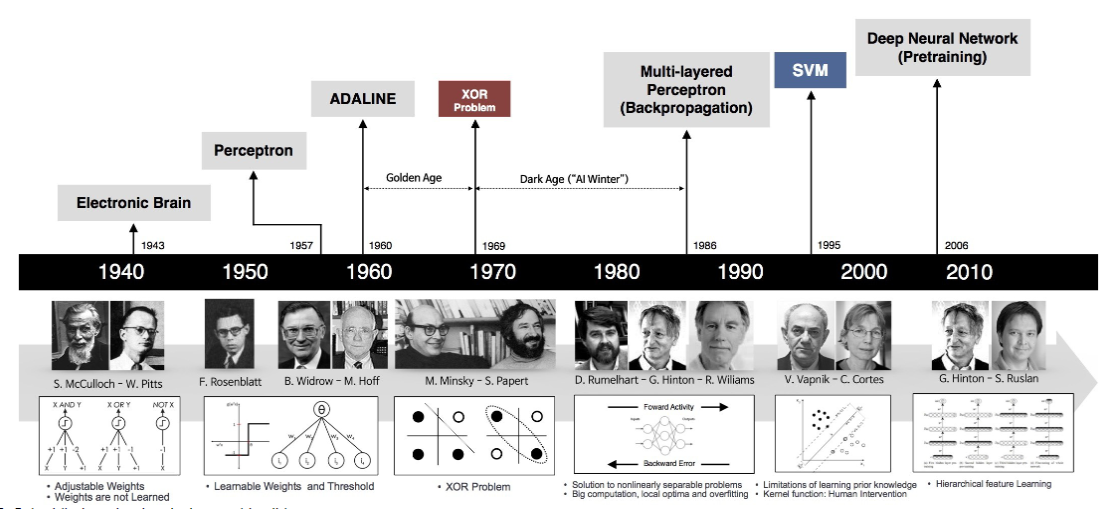
\includegraphics[width=\textwidth]{figures/timeline.png}
\end{center}
\end{frame}

% --- Deep Learning in Economics and Finance ---
\begin{frame}{Deep Learning in Economics and Finance}
\small
\begin{columns}[T]
\column{0.48\textwidth}
\textbf{Forecasting \& Nowcasting}
\begin{itemize}\setlength{\itemsep}{1pt}
    \item GDP nowcasting from high-frequency data
    \item Inflation forecasting with nonlinear models
    \item Yield curve modeling and term structure
\end{itemize}

\vspace{0.2cm}
\textbf{Text \& Communication}
\begin{itemize}\setlength{\itemsep}{1pt}
    \item NLP on central bank minutes and speeches
    \item Sentiment analysis of financial news
    \item Measuring policy uncertainty
\end{itemize}

\column{0.48\textwidth}
\textbf{Financial Stability \& Supervision}
\begin{itemize}\setlength{\itemsep}{1pt}
    \item Fraud and anomaly detection
    \item Credit risk scoring
    \item Stress testing and scenario generation
\end{itemize}

\vspace{0.2cm}
\textbf{Structural Models}
\begin{itemize}\setlength{\itemsep}{1pt}
    \item Solving and estimating structural models (DSGE, OLG, heterogeneous agents)
    \item Overcoming the curse of dimensionality
    \item NN-based surrogates for equilibrium computation
\end{itemize}
\end{columns}

\vspace{0.2cm}
\begin{center}
{\footnotesize \emphc{This course} focuses on the last category, using deep learning as a computational tool for economic modeling.}
\end{center}
\end{frame}

% --- Slide 11: Useful Materials ---
\begin{frame}{Useful Materials}
\begin{columns}[T]
\column{0.42\textwidth}
\begin{center}
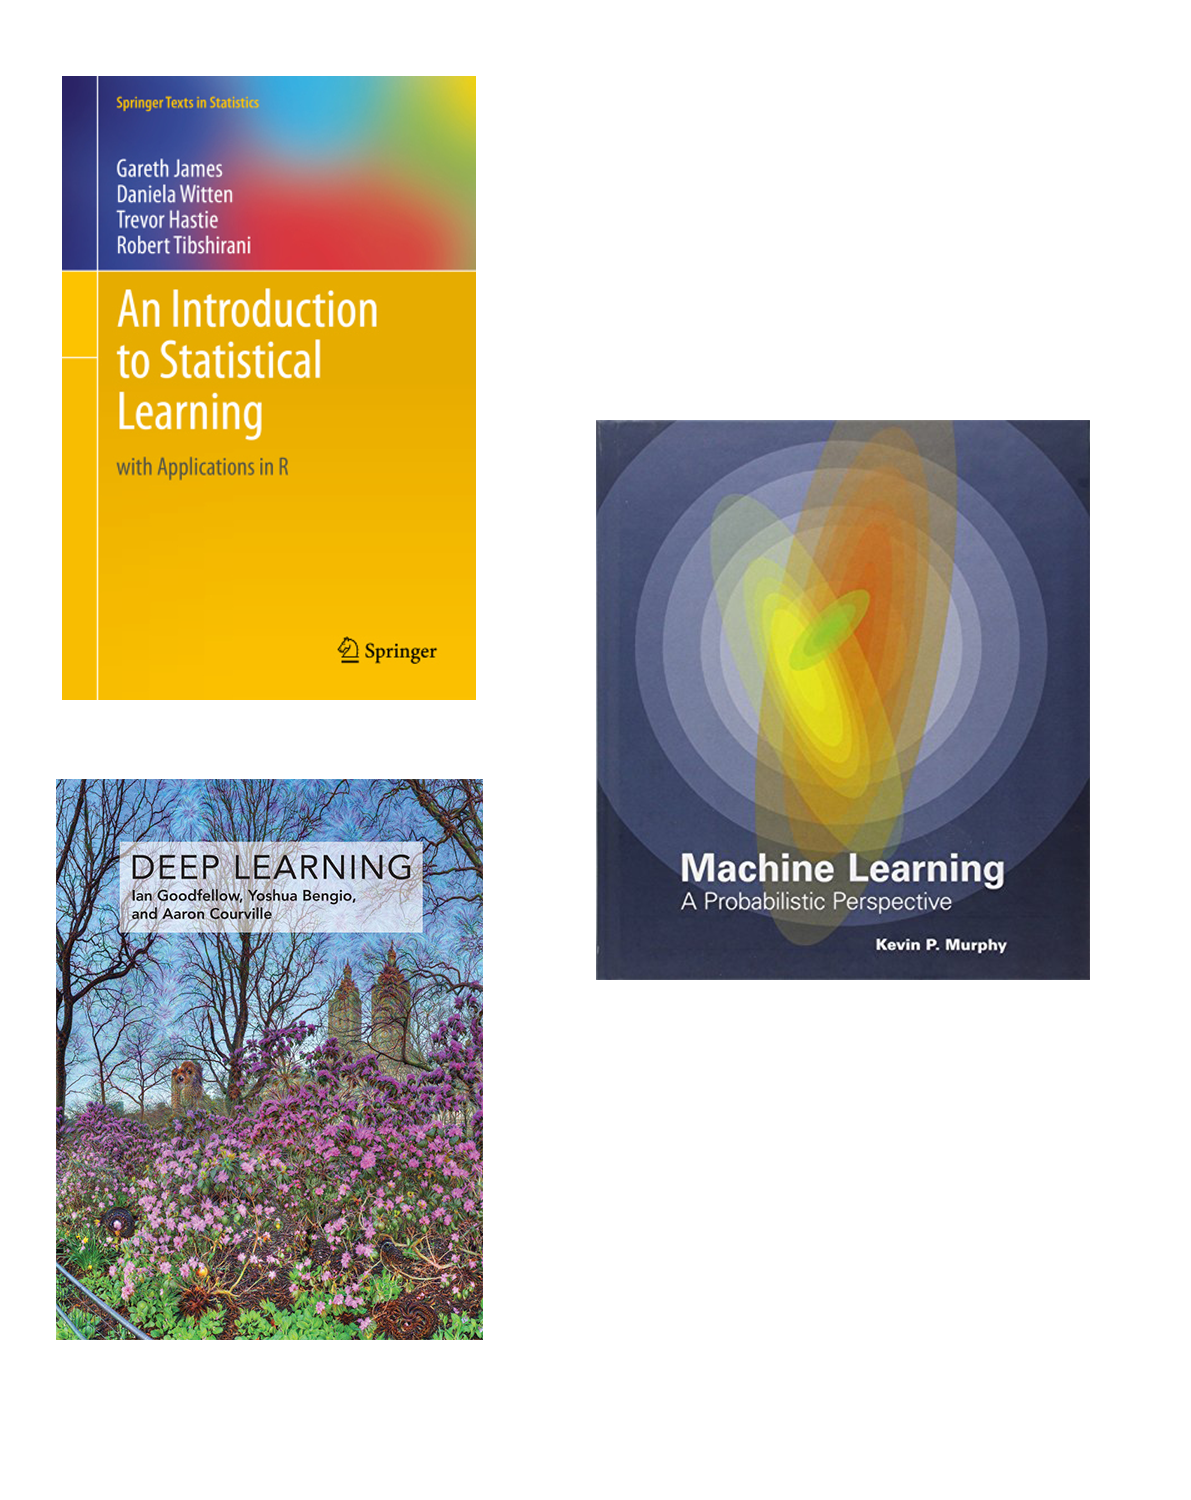
\includegraphics[width=0.9\textwidth]{figures/books1.png}
\end{center}

\column{0.55\textwidth}
\begin{enumerate}
    \item \textbf{I.\ Goodfellow, Y.\ Bengio, A.\ Courville} (2016).
          \textit{Deep Learning}. MIT Press.
          \hfill \url{https://www.deeplearningbook.org}

    \vspace{0.3cm}
    \item \textbf{K.\ P.\ Murphy} (2022).
          \textit{Probabilistic Machine Learning: An Introduction}. MIT Press.

    \vspace{0.3cm}
    \item \textbf{G.\ James et al.} (2021).
          \textit{An Introduction to Statistical Learning} (ISLR). Springer.
          \hfill \url{https://www.statlearning.com}
\end{enumerate}
\end{columns}
\end{frame}

% --- Slide 12: Why Deep Learning Now? ---
\begin{frame}{Why Deep Learning Now?}
Neural networks date back to the 1940s.  Three developments made them practical:

\vspace{0.4cm}
\begin{center}
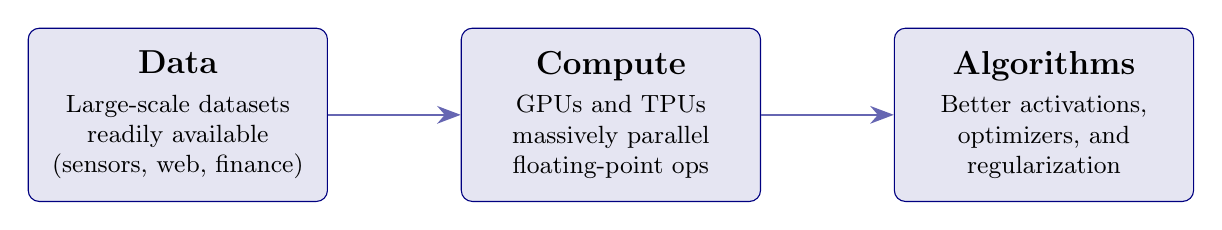
\begin{tikzpicture}[
    box/.style={rectangle, draw=uzhblue, fill=uzhblue!10, rounded corners=4pt,
                minimum width=3.8cm, minimum height=2.2cm, align=center, font=\small},
    arr/.style={-{Stealth[length=3mm]}, thick, uzhblue!60}
]
    \node[box] (data) at (0,0) {\textbf{\large Data}\\[3pt]Large-scale datasets\\readily available\\(sensors, web, finance)};
    \node[box] (hw) at (5.5,0) {\textbf{\large Compute}\\[3pt]GPUs and TPUs\\massively parallel\\floating-point ops};
    \node[box] (sw) at (11,0) {\textbf{\large Algorithms}\\[3pt]Better activations,\\optimizers, and\\regularization};

    \draw[arr] (data) -- (hw);
    \draw[arr] (hw) -- (sw);
\end{tikzpicture}
\end{center}

\vspace{0.3cm}
{\small Key milestones: Perceptron (1958), Backpropagation (1986), Deep CNN (1995), AlexNet (2012), Transformers (2017), ChatGPT (2022).}
\end{frame}


% ============================================================================
% PART 2: MACHINE LEARNING FOUNDATIONS
% ============================================================================

\section{Machine Learning Foundations}

% --- Section Divider ---
\begin{frame}{}
\begin{center}
{\Huge \textcolor{uzhblue}{Part I}}\\[0.8em]
{\LARGE Machine Learning Foundations}
\end{center}
\end{frame}

% --- Slide 7: What is Machine Learning? ---
\begin{frame}{What is Machine Learning?}
\begin{columns}[T]
\column{0.45\textwidth}
\begin{center}
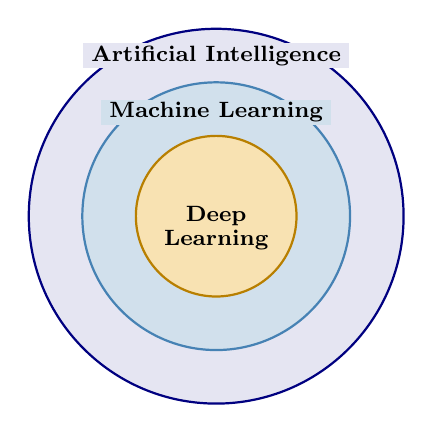
\begin{tikzpicture}[scale=0.85]
    % Concentric circles: AI > ML > DL
    \fill[uzhblue!10] (0,0) circle (2.8cm);
    \fill[softblue!25] (0,0) circle (2.0cm);
    \fill[softorange!30] (0,0) circle (1.2cm);
    \draw[uzhblue, thick] (0,0) circle (2.8cm);
    \draw[softblue, thick] (0,0) circle (2.0cm);
    \draw[softorange!80!black, thick] (0,0) circle (1.2cm);
    \node[font=\footnotesize\bfseries] at (0,0) {Deep};
    \node[font=\footnotesize\bfseries] at (0,-0.35) {Learning};
    \node[font=\footnotesize\bfseries, fill=softblue!25, inner xsep=3pt, inner ysep=1pt] at (0,1.55) {Machine Learning};
    \node[font=\footnotesize\bfseries, fill=uzhblue!10, inner xsep=3pt, inner ysep=1pt] at (0,2.4) {Artificial Intelligence};
\end{tikzpicture}
\end{center}

\column{0.52\textwidth}
\textbf{Classical programming:}

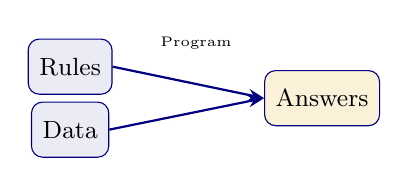
\begin{tikzpicture}[
    box/.style={rectangle, draw=uzhblue, fill=uzhblue!8, rounded corners,
                minimum height=7mm, font=\small, inner sep=4pt},
    arr/.style={-{Stealth[length=2mm]}, thick, uzhblue}]
    \node[box] (r) at (0,0) {Rules};
    \node[box] (d) at (0,-0.8) {Data};
    \node[box, fill=softorange!15] (a) at (3.2,-0.4) {Answers};
    \draw[arr] (r.east) -- (a.west);
    \draw[arr] (d.east) -- (a.west);
    \node[font=\tiny, above] at (1.6, 0.1) {Program};
\end{tikzpicture}

\vspace{0.4cm}
\textbf{Machine learning:}

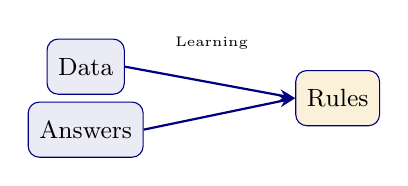
\begin{tikzpicture}[
    box/.style={rectangle, draw=uzhblue, fill=uzhblue!8, rounded corners,
                minimum height=7mm, font=\small, inner sep=4pt},
    arr/.style={-{Stealth[length=2mm]}, thick, uzhblue}]
    \node[box] (d) at (0,0) {Data};
    \node[box] (a) at (0,-0.8) {Answers};
    \node[box, fill=softorange!15] (r) at (3.2,-0.4) {Rules};
    \draw[arr] (d.east) -- (r.west);
    \draw[arr] (a.east) -- (r.west);
    \node[font=\tiny, above] at (1.6, 0.1) {Learning};
\end{tikzpicture}
\end{columns}
\end{frame}

% --- Slide 8: Types of ML ---
\begin{frame}{Types of Machine Learning}
\begin{columns}[T]
\column{0.32\textwidth}
\begin{block}{\centering Supervised}
    Given labeled pairs $\{(\x^{(i)}, y^{(i)})\}_{i=1}^{m}$, learn a mapping $h:\mathcal{X}\to\mathcal{Y}$.

    \vspace{0.3em}
    \textbf{Regression:} $y\in\R$\\
    \textbf{Classification:} $y\in\{0,1,\dots,K\}$
\end{block}

\column{0.32\textwidth}
\begin{block}{\centering Unsupervised}
    Given only $\{\x^{(i)}\}_{i=1}^{m}$, discover hidden structure.

    \vspace{0.3em}
    \textbf{Clustering:} group similar points\\
    \textbf{Dim.\ reduction:} compress features
\end{block}

\column{0.32\textwidth}
\begin{block}{\centering Reinforcement}
    An agent acts in an environment, receives rewards, and learns a policy $\pi$.

    \vspace{0.3em}
    \textbf{Policy:} $a_t = \pi(s_t)$\\
    \textbf{Goal:} maximize $\sum_t \gamma^t r_t$
\end{block}
\end{columns}

\vspace{0.5cm}
\begin{center}
{\small This course covers \textbf{both} paradigms: we begin with the \emph{supervised} pipeline (model, loss, optimizer)\\
and then build on it for the \emph{unsupervised} methods at the heart of the course (DEQNs, PINNs).}
\end{center}
\end{frame}

% --- Slide 9: Supervised Regression ---
\begin{frame}{Supervised Learning: Regression}
\begin{columns}[T]
\column{0.52\textwidth}
\textbf{Goal:} predict a continuous target $y\in\R$ from features $\x\in\R^d$.

\vspace{0.3cm}
\textbf{Setup:}
\begin{itemize}
    \item Training data: $\{(\x^{(i)}, y^{(i)})\}_{i=1}^{m}$
    \item Model (hypothesis): $\hat{y} = h(\x;\bm{\theta})$
    \item Parameters $\bm{\theta}$ learned from data
\end{itemize}

\vspace{0.3cm}
\textbf{Linear example:}
\[
    h_{\bm{\theta}}(x) = \theta_0 + \theta_1 x
\]

\column{0.45\textwidth}
\begin{center}
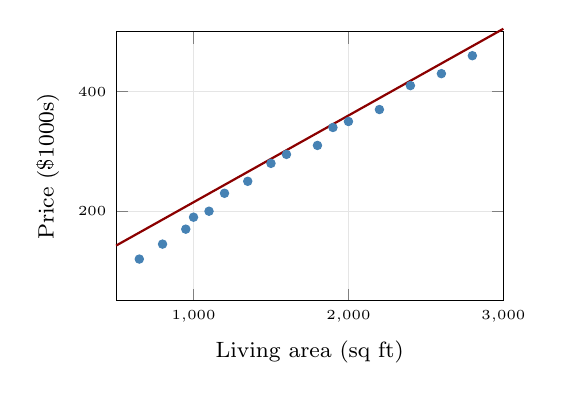
\begin{tikzpicture}
\begin{axis}[
    width=6.5cm, height=5cm,
    xlabel={Living area (sq ft)},
    ylabel={Price (\$1000s)},
    xlabel style={font=\footnotesize},
    ylabel style={font=\footnotesize},
    tick label style={font=\tiny},
    xmin=500, xmax=3000, ymin=50, ymax=500,
    grid=major, grid style={gray!20},
    clip=false
]
    % Scatter data
    \addplot[only marks, mark=*, mark size=1.5pt, softblue] coordinates {
        (650,120) (800,145) (950,170) (1000,190) (1100,200) (1200,230)
        (1350,250) (1500,280) (1600,295) (1800,310) (1900,340)
        (2000,350) (2200,370) (2400,410) (2600,430) (2800,460)
    };
    % Regression line
    \addplot[thick, darkred, domain=500:3000, samples=2]{70 + 0.145*x};
\end{axis}
\end{tikzpicture}
\end{center}
\end{columns}
\end{frame}

% --- Slide 10: Classification ---
\begin{frame}{Supervised Learning: Classification}
\begin{columns}[T]
\column{0.50\textwidth}
\textbf{Goal:} assign an input $\x$ to one of $K$ classes.

\vspace{0.3cm}
\textbf{Example -- Credit scoring:}
\begin{itemize}
    \item Features: income, savings
    \item Labels: low-risk / high-risk
    \item Decision boundary separates classes
\end{itemize}

\vspace{0.3cm}
A simple linear rule:
\[
    \text{if } \w^\top \x + b > 0 \;\Rightarrow\; \text{low-risk}
\]

\column{0.47\textwidth}
\begin{center}
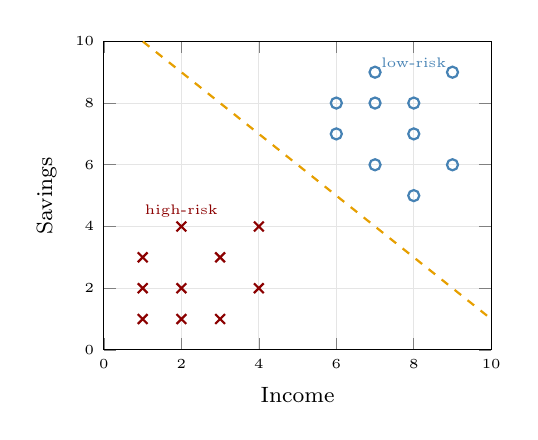
\begin{tikzpicture}
\begin{axis}[
    width=6.5cm, height=5.5cm,
    xlabel={Income}, ylabel={Savings},
    xlabel style={font=\footnotesize},
    ylabel style={font=\footnotesize},
    tick label style={font=\tiny},
    xmin=0, xmax=10, ymin=0, ymax=10,
    grid=major, grid style={gray!20},
]
    % Low-risk (blue)
    \addplot[only marks, mark=o, mark size=2pt, softblue, thick] coordinates {
        (6,7) (7,6) (8,5) (7,8) (8,7) (9,6) (6,8) (8,8) (9,9) (7,9)
    };
    % High-risk (red)
    \addplot[only marks, mark=x, mark size=2.5pt, darkred, thick] coordinates {
        (1,2) (2,1) (3,3) (2,4) (1,3) (4,2) (3,1) (2,2) (4,4) (1,1)
    };
    % Decision boundary
    \addplot[thick, softorange, dashed, domain=0:10, samples=2]{11-x};
    \node[font=\tiny, softblue] at (axis cs:8,9.3) {low-risk};
    \node[font=\tiny, darkred] at (axis cs:2,4.5) {high-risk};
\end{axis}
\end{tikzpicture}
\end{center}
\end{columns}
\end{frame}

% --- Slide 11: The ML Recipe ---
\begin{frame}{The Machine Learning Recipe}
Every machine learning algorithm follows the same three steps:

\vspace{0.5cm}
\begin{center}
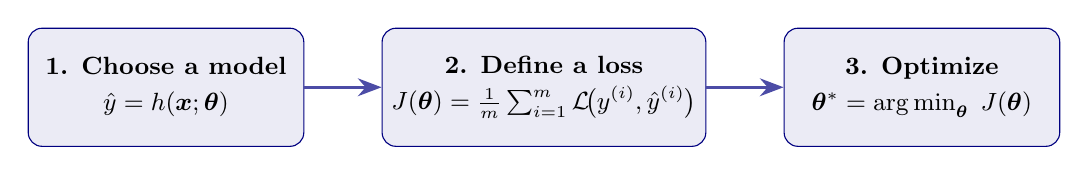
\begin{tikzpicture}[
    mlstep/.style={rectangle, draw=uzhblue, fill=uzhblue!8, rounded corners=5pt,
                 minimum width=3.5cm, minimum height=1.5cm, align=center, font=\small},
    arr/.style={-{Stealth[length=3mm]}, very thick, uzhblue!70}
]
    \node[mlstep] (m) at (0,0) {\textbf{1. Choose a model}\\[2pt]$\hat{y} = h(\x;\bm{\theta})$};
    \node[mlstep] (l) at (4.8,0) {\textbf{2. Define a loss}\\[2pt]$J(\bm{\theta}) = \frac{1}{m}\sum_{i=1}^{m}\mathcal{L}\!\big(y^{(i)},\hat{y}^{(i)}\big)$};
    \node[mlstep] (o) at (9.6,0) {\textbf{3. Optimize}\\[2pt]$\bm{\theta}^{*} = \argmin_{\bm{\theta}}\; J(\bm{\theta})$};

    \draw[arr] (m) -- (l);
    \draw[arr] (l) -- (o);
\end{tikzpicture}
\end{center}

\vspace{0.3cm}
\begin{block}{Cost function example (supervised regression: Mean Squared Error)}
\[
    J(\bm{\theta}) \;=\; \frac{1}{2m}\sum_{i=1}^{m}\!\big(h_{\bm{\theta}}(\x^{(i)}) - y^{(i)}\big)^{2}
\]
\end{block}
{\footnotesize\emphc{Same recipe, different loss.}  DEQNs and PINNs (later chapters) replace step~2 by an Euler-equation or PDE residual; steps~1 and~3 are unchanged.}
\end{frame}

% --- Slide 12: Supervised Learning Pipeline ---
\begin{frame}{Supervised Learning Pipeline}
\begin{center}
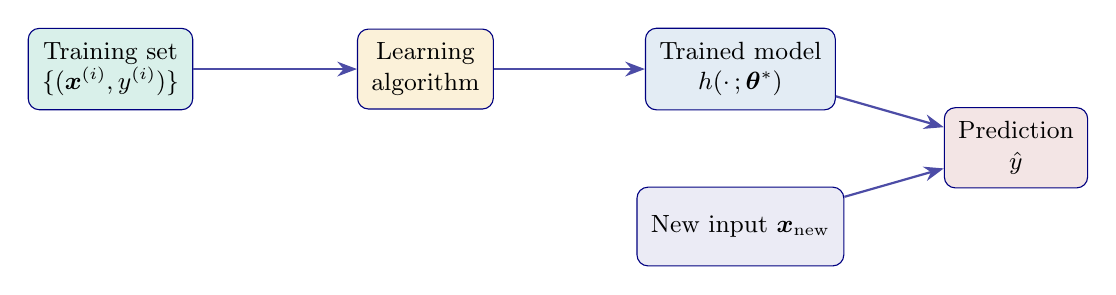
\begin{tikzpicture}[
    box/.style={rectangle, draw=uzhblue, fill=uzhblue!8, rounded corners=4pt,
                minimum height=1cm, align=center, font=\small, inner sep=5pt},
    arr/.style={-{Stealth[length=2.5mm]}, thick, uzhblue!70}
]
    \node[box, fill=softgreen!15] (data) at (0,0) {Training set\\$\{(\x^{(i)}, y^{(i)})\}$};
    \node[box, fill=softorange!15] (algo) at (4,0) {Learning\\algorithm};
    \node[box, fill=softblue!15] (model) at (8,0) {Trained model\\$h(\cdot\,;\bm{\theta}^{*})$};
    \node[box] (xnew) at (8,-2) {New input $\x_{\mathrm{new}}$};
    \node[box, fill=darkred!10] (pred) at (11.5,-1) {Prediction\\$\hat{y}$};

    \draw[arr] (data) -- (algo);
    \draw[arr] (algo) -- (model);
    \draw[arr] (model) -- (pred);
    \draw[arr] (xnew) -- (pred);
\end{tikzpicture}
\end{center}

\vspace{0.5cm}
\textbf{Computationally, we need:}
\begin{itemize}
    \item Data (labeled examples)
    \item Linear algebra and automatic differentiation
    \item An optimization routine (gradient-based)
\end{itemize}
\end{frame}

% --- Slide 13: Unsupervised Learning ---
\begin{frame}{Unsupervised Learning}
\begin{columns}[T]
\column{0.50\textwidth}
No labels, only inputs $\{\x^{(i)}\}_{i=1}^{m}$. The goal is to discover hidden structure.

\vspace{0.3cm}
\textbf{Clustering:} partition data into groups of similar points (e.g., customer segmentation, image compression).

\vspace{0.3cm}
\textbf{Dimensionality reduction:} project high-dimensional data to a lower-dimensional space (e.g., PCA, autoencoders).

\column{0.47\textwidth}
\begin{center}
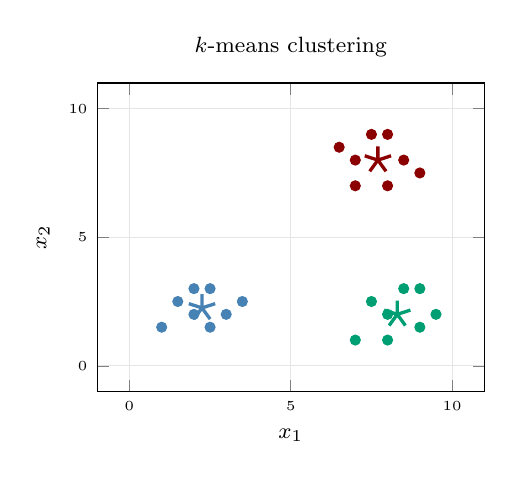
\begin{tikzpicture}
\begin{axis}[
    width=6.5cm, height=5.5cm,
    xlabel={$x_1$}, ylabel={$x_2$},
    xlabel style={font=\footnotesize},
    ylabel style={font=\footnotesize},
    tick label style={font=\tiny},
    xmin=-1, xmax=11, ymin=-1, ymax=11,
    grid=major, grid style={gray!20},
    title={\footnotesize $k$-means clustering},
    title style={font=\footnotesize},
]
    % Cluster 1 (blue)
    \addplot[only marks, mark=*, mark size=1.8pt, softblue] coordinates {
        (2,2) (2.5,1.5) (1.5,2.5) (3,2) (2,3) (1,1.5) (2.5,3) (3.5,2.5)
    };
    % Cluster 2 (red)
    \addplot[only marks, mark=*, mark size=1.8pt, darkred] coordinates {
        (7,8) (8,7) (7.5,9) (8.5,8) (9,7.5) (7,7) (8,9) (6.5,8.5)
    };
    % Cluster 3 (green)
    \addplot[only marks, mark=*, mark size=1.8pt, softgreen] coordinates {
        (8,2) (9,1.5) (7.5,2.5) (8.5,3) (9.5,2) (7,1) (8,1) (9,3)
    };
    % Centroids
    \addplot[only marks, mark=star, mark size=5pt, softblue, very thick] coordinates {(2.25,2.25)};
    \addplot[only marks, mark=star, mark size=5pt, darkred, very thick] coordinates {(7.7,8)};
    \addplot[only marks, mark=star, mark size=5pt, softgreen, very thick] coordinates {(8.3,2)};
\end{axis}
\end{tikzpicture}
\end{center}
\end{columns}
\end{frame}

% --- Slide 14: Reinforcement Learning ---
\begin{frame}{Reinforcement Learning (Brief)}
\begin{center}
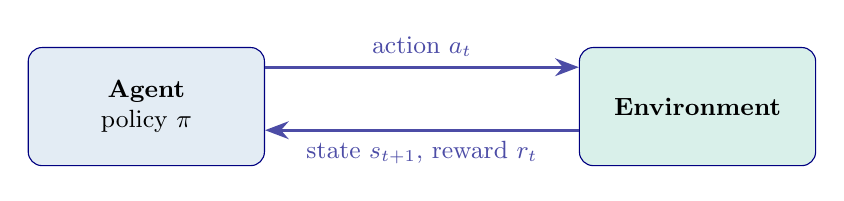
\begin{tikzpicture}[
    box/.style={rectangle, draw=uzhblue, fill=uzhblue!8, rounded corners=5pt,
                minimum width=3cm, minimum height=1.5cm, align=center, font=\small},
    arr/.style={-{Stealth[length=3mm]}, very thick, uzhblue!70}
]
    \node[box, fill=softblue!15] (agent) at (0,0) {\textbf{Agent}\\policy $\pi$};
    \node[box, fill=softgreen!15] (env) at (7,0) {\textbf{Environment}};

    \draw[arr] ([yshift=5mm]agent.east) -- node[above, font=\small]{action $a_t$} ([yshift=5mm]env.west);
    \draw[arr] ([yshift=-3mm]env.west) -- node[below, font=\small]{state $s_{t+1}$, reward $r_t$} ([yshift=-3mm]agent.east);
\end{tikzpicture}
\end{center}

\vspace{0.5cm}
\begin{itemize}
    \item The agent learns a policy $\pi(a\mid s)$ to maximize cumulative discounted reward $\sum_{t=0}^{\infty}\gamma^t r_t$.
    \item No explicit supervision, only delayed reward signals.
    \item Applications: game playing (AlphaGo), robotics, portfolio optimization.
\end{itemize}

\vspace{0.3cm}
{\small We will not cover RL in this course, but the neural network tools you learn here are the building blocks for deep RL.}
\end{frame}

% --- Slide 53: Questions ---
\begin{frame}{}
\begin{columns}[c]
\column{0.45\textwidth}
\begin{center}
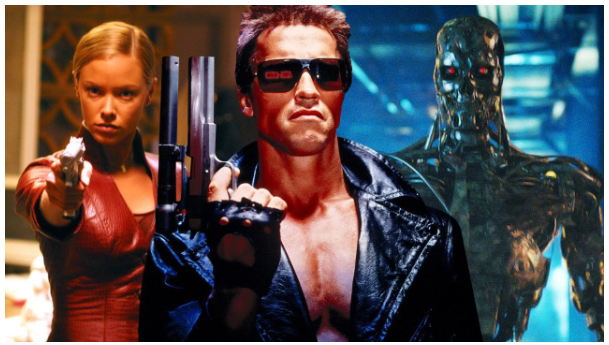
\includegraphics[width=0.85\textwidth]{figures/quest.png}
\end{center}

\column{0.50\textwidth}
\begin{center}
{\Huge \textcolor{uzhblue}{\textbf{Questions?}}}

\vspace{0.8cm}
{\large Simon Scheidegger}\\[4pt]
{\small HEC, University of Lausanne}\\[4pt]
\url{https://sischei.github.io}

\vspace{0.6cm}
{\small Materials:~~\url{https://github.com/sischei/Deep_Learning_for_Solving_And_Estimating_Dynamic_Economic_Models}}
\end{center}
\end{columns}
\end{frame}

\end{document}
